\documentclass[a4paper,12pt]{article}
\usepackage[utf8]{inputenc}
\usepackage[IL2]{fontenc}
\usepackage{listings}
\usepackage{amssymb}
\usepackage{amsmath}
\usepackage{url}
\usepackage{graphicx}
\usepackage[czech]{babel}
\title{Kolektivní investování}
\author{Marek Bryša, Jan Kovář}
\date{Brno, \today}
\begin{document}
\maketitle

\section{Úvod}

\section{Charakteristika konkrétních fondů v ČR}
	\subsection{AXA investiční společnost, a.s.}
		Francouzská skupina AXA je druhým největším správcem fondů v Evropě.\cite{axa_about} Její produkty mají v České republice nulové vstupní poplatky, ale klient hradí správní poplatky a výstupní v případě ukončení investice za kratší dobu než 5 let. Kompletní přehled poplatků je uveden v příloze \ref{axa}.
		
		Pro drobné investory jsou určeny všechny fondy se vstupní investicí 5~000 Kč. Výjimkou je AXA Corporate Fund, který má minimální vstupní investici 1~000~000 Kč a následnou 500~000 Kč.
		
		\subsubsection{AXA CZK Konto}
			AXA CZK Konto je otevřený podílový fond, který byl do 31.12.2011 klasifikován jako fond peněžního trhu, od 1.1.2012 se podle metodiky AKAT ČR jedná o smíšený fond.
			\begin{quote}
				Cílem investiční strategie je poskytnout podílníkům růst hodnoty jejich investice za podmínky, že celkový rizikový profil fondu minimalizuje možnost ztráty v horizontu 6 měsíců. Cíle je dosahováno investicemi do široce diverzifikovaného portfolia cenných papírů s fixním nebo variabilním úrokovým výnosem a aktivním řízením úrokového rizika.\footnote{\url{http://www.axa.cz/lide/podilove-fondy/czk-konto/popis}}
			\end{quote}
			
			Doporučeným investičním horizontem je minimálně 6 měsícu. Fond je vhodný pro investora s nízkou tolerancí k riziku, který neočekává vysoký výnos.
			
			Graf zhodnocení fondu je uveden v obrázku \ref{axa_czk_konto}. Fond připsal za 5 let 10.07\%, v průměru tedy 2.05\% ročně, přičemž za poslední rok 0.8\%. Po odečtení správcovského poplatku je čistý roční výnos 1.55\%, což je výrazně méně než nabízely a nabízejí spořící účty v bankách.
			\begin{figure}[h!]
				\label{axa_czk_konto}

		  	\centering
				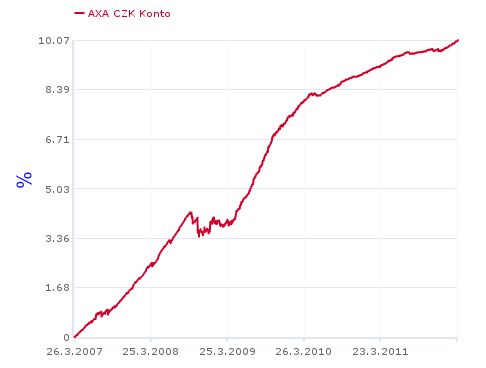
\includegraphics[width=0.6\textwidth]{axa_czk_konto.png}			
				\caption{Graf zhodnocení AXA CZK Konto za 5 let zdroj: http://www.axa.cz/fondy/porovnani/podilove.aspx?fund=29}
			\end{figure}

\newpage	
\appendix
\section{Poplatky AXA investiční společnost \cite{axa_cite}}
\label{axa}	
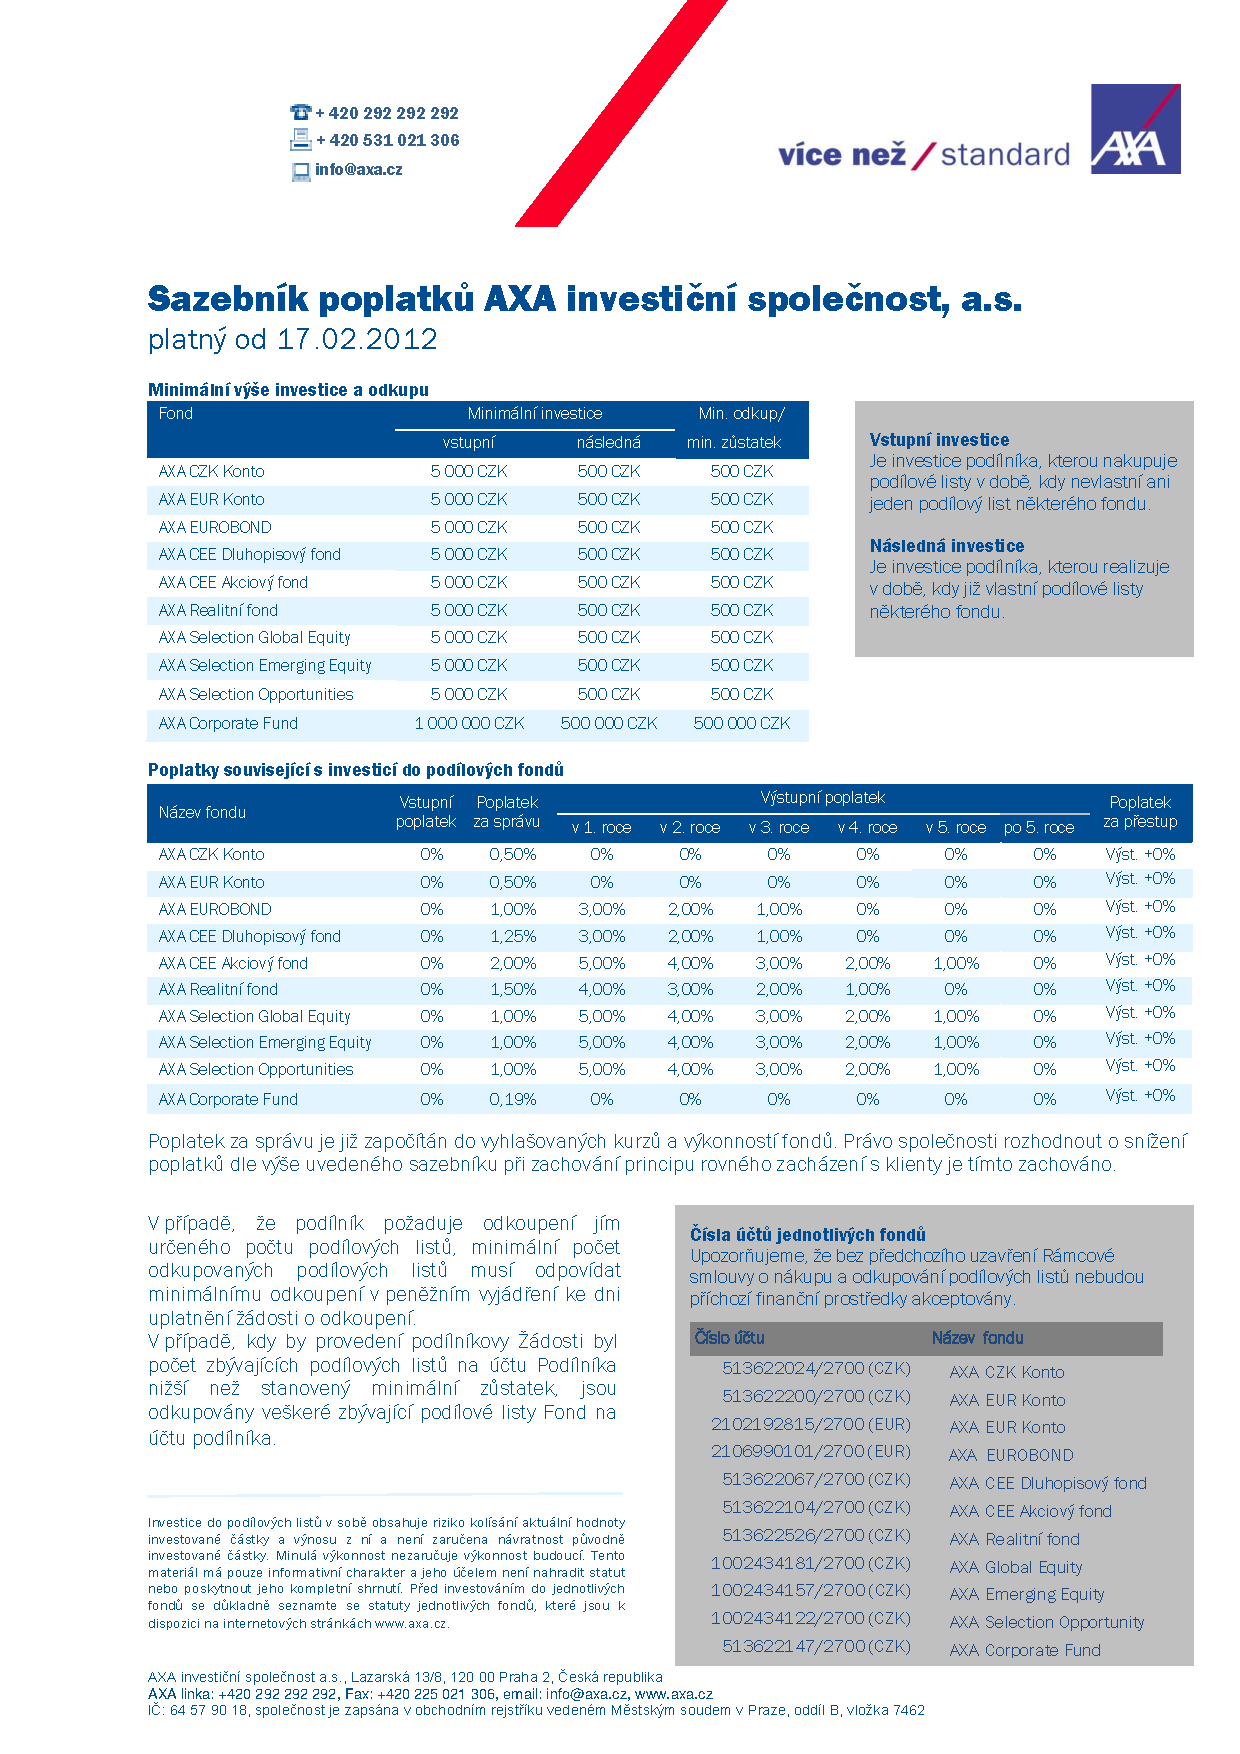
\includegraphics[width=1.0\textwidth]{axa.pdf}
\renewcommand{\bibname}{Seznam použité literatury}
\begin{thebibliography}{9}
\addcontentsline{toc}{chapter}{Seznam použité literatury}
\thispagestyle{plain}

\bibitem{camsky} ČÁMSKÝ, František. \emph{Teorie portfolia.} 2. přeprac. a rozš. vyd. Brno : Masarykova univerzita, 2007. 115 s. ISBN 9788021042520.

\bibitem{axa_about}
Leták Podílové fondy AXA, [cit. 2012-03-23], Dostupné z WWW:  \url{http://www.axa.cz/getattachment/59ed8936-2745-409d-952b-801213d54a2d/Letak-Podilove-fondy}


\bibitem{axa_cite}
Sazebník poplatků AXA investiční společnost, a.s., [cit. 2012-03-23], Dostupné z WWW:  \url{http://www.axa.cz/getattachment/edb1852e-a78d-4c80-9515-55f0f1db5953/Sazebnik-poplatku}
\end{thebibliography}
\end{document}